%%\documentclass[referee,sn-basic]{sn-jnl}% referee option is meant for double line spacing

%%=======================================================%%
%% to print line numbers in the margin use lineno option %%
%%=======================================================%%

%%\documentclass[lineno,sn-basic]{sn-jnl}% Basic Springer Nature Reference Style/Chemistry Reference Style

%%======================================================%%
%% to compile with pdflatex/xelatex use pdflatex option %%
%%======================================================%%

%%\documentclass[pdflatex,sn-basic]{sn-jnl}% Basic Springer Nature Reference Style/Chemistry Reference Style


%%Note: the following reference styles support Namedate and Numbered referencing. By default the style follows the most common style. To switch between the options you can add or remove “Numbered” in the optional parenthesis. 
%%The option is available for: sn-basic.bst, sn-vancouver.bst, sn-chicago.bst, sn-mathphys.bst. %  
 
\documentclass[sn-nature]{sn-jnl}% Style for submissions to Nature Portfolio journals
%%\documentclass[sn-basic]{sn-jnl}% Basic Springer Nature Reference Style/Chemistry Reference Style
%%\documentclass[sn-mathphys,Numbered]{sn-jnl}% Math and Physical Sciences Reference Style
%%\documentclass[sn-aps]{sn-jnl}% American Physical Society (APS) Reference Style
%%\documentclass[sn-vancouver,Numbered]{sn-jnl}% Vancouver Reference Style
%%\documentclass[sn-apa]{sn-jnl}% APA Reference Style 
%%\documentclass[sn-chicago]{sn-jnl}% Chicago-based Humanities Reference Style
%%\documentclass[default]{sn-jnl}% Default
%%\documentclass[default,iicol]{sn-jnl}% Default with double column layout

%%%% Standard Packages
%%<additional latex packages if required can be included here>

\usepackage{graphicx}%
\usepackage{multirow}%
\usepackage{amsmath,amssymb,amsfonts}%
\usepackage{amsthm}%
\usepackage{mathrsfs}%
\usepackage[title]{appendix}%
\usepackage{xcolor}%
\usepackage{textcomp}%
\usepackage{manyfoot}%
\usepackage{booktabs}%
\usepackage{algorithm}%
\usepackage{algorithmicx}%
\usepackage{algpseudocode}%
\usepackage{listings}%
%%%%


%\jyear{2021}%


\raggedbottom
%%\unnumbered% uncomment this for unnumbered level heads

\begin{document}

\title[MASH]{MASH: a toolbox for Multi-ancestry SNP-heritability simulation and estimation}

\author[1]{\fnm{Christian} \sur{Coffman}\email{coffm049@umn.edu}}

\author[2]{\fnm{Seon-Kyeong} \sur{Jang}}\email{jangx303@umn.edu}
\equalcont{These authors contributed equally to this work.}

\author*[1]{\fnm{Saonli} \sur{Basu}}\email{saonli@umn.edu}
\equalcont{These authors contributed equally to this work.}

\affil*[1]{\orgdiv{Division of Biostatistics}, \orgname{University of Minnesota}, \orgaddress{\street{Street}, \city{Minneapolis}, \postcode{100190}, \state{Minnesota}, \country{USA}}}

\affil[2]{\orgdiv{Department of Psychology}, \orgname{University of Minnesota}, \orgaddress{\street{Street}, \city{Minneapolis}, \postcode{55455}, \state{Minnesota}, \country{USA}}}


%%================================%%
%% Sample for structured abstract %%
%%================================%%

% Abstract <350 words, minimize abbreviations, no citations, 
% Background 
% The context at purpose of the study
\begin{abstract}
\noindent \textbf{Background:} Simulating quantitative phenotypes from multiple ancestries is essential for assessing and developing statistical methods in population genetics and genetic epidemiology. However, the availability of standardized tools for such simulations has been limited. The MASH toolbox is a powerful and user-friendly tool to fill this gap.

\noindent \textbf{Results:} The MASH toolbox implements a simulation class that allows users to control the number and distribution of genetic ancestries across sites, incorporate confounding covariates such as site effects, and simulate SNP effects based on observed allele frequencies. The toolbox offers flexibility in controlling heritability either for each genetic ancestry separately or collectively. Additionally, it provides tools for adjusting site effects, meta-analysis estimation, and REML estimation using GCTA for SNP-heritability estimation all within Python. Simulation results demonstrate the ability of the toolbox to generate minimally complex, realistic simulations that capture the diversity and relationships among different populations, while the estimators included in the toolbox are shown to be unbiased through comprehensive simulation studies.

\noindent \textbf{Conclusions:} The MASH toolbox fills the gap in standardized tools for simulating quantitative phenotypes from multiple ancestries in a user-friendly manner. Its modular design allows for easy extensibility to accommodate specific use cases, and the inclusion of additional tools for removing site effects and SNP-heritability estimation further enhances its utility. By providing minimally complex, realistic simulations and unbiased estimators, the MASH toolbox empowers researchers to explore and understand the genetic contributions to phenotypic variation in multi-ancestry populations. We anticipate that the toolbox will greatly facilitate the assessment of statistical methods and advance research in population genetics and genetic epidemiology.

\end{abstract}\keywords{SNP-heritability, scanner effects, ABCD, method of moments}

%%\pacs[JEL Classification]{D8, H51}

%%\pacs[MSC Classification]{35A01, 65L10, 65L12, 65L20, 65L70}

\maketitle

% Aim for 3300 words

\section{Introduction}\label{sec:intro}
% Motivation: Simulating quantitative phenotypes from multiple ancestries is essential for assessing and developing statistical methods in population genetics and genetic epidemiology.
% Existing gap: Currently, there is a lack of standardized tools that enable easy simulation of multi-ancestry, multi-site data, hindering progress in this field.
% Toolbox description: We present the MASH toolbox, a powerful and user-friendly tool for simulating and estimating quantitative phenotypes from multiple ancestries.
% Simulating multi-site studies: MASH is specifically designed to create realistic simulations for multi-site studies, allowing for the exploration of correlations between site membership and genetic ancestry.
% SNP effects based on frequency: MASH incorporates the observed frequency of SNPs to simulate their effects, aligning with current genetic theories and providing more realistic simulations.
% Broad applicability: Researchers using MASH can simulate phenotypes across diverse populations, including datasets such as the "thousand genomes," enabling comprehensive analysis and assessment of methods.
The study of genetic variation and its impact on phenotypic traits is crucial for understanding the genetic basis of complex diseases and population diversity. In multi-ancestry studies, it is essential to simulate realistic phenotypes that capture the complexity and diversity of different genetic ancestries, while also considering confounding covariates such as site effects. However, the availability of standardized tools for generating such simulations has been limited, impeding progress in the field.

In this paper, we introduce the MASH toolbox, a comprehensive and user-friendly statistical toolbox designed to address the need for simulation of quantitative phenotypes from multiple ancestries in a multi-site context. The MASH toolbox fills a critical gap in the field by providing researchers with a powerful and versatile tool for creating minimally complex, yet realistic simulations that incorporate population-specific allele frequencies, genetic relatedness, and confounding covariates. The toolbox follows an object-oriented paradigm implemented in Python, allowing for easy customization and extensibility to accommodate specific use cases.

The MASH toolbox offers a range of features to simulate and estimate quantitative phenotypes. Users have control over the number and distribution of genetic ancestries across sites, allowing for the creation of diverse multi-ancestry scenarios. Additionally, the toolbox allows for the incorporation of confounding covariates, such as site effects, which is critical in multi-site studies. Users can simulate SNP effects based on observed allele frequencies, aligning with current genetic theories. Furthermore, the toolbox provides estimators for adjusting site effects, conducting meta-analysis, and estimating SNP-heritability using REML estimation with GCTA. These estimators have been verified through comprehensive simulation studies, demonstrating their unbiasedness and suitability for analyzing multi-ancestry datasets.

By offering a standardized and accessible platform for simulating and estimating quantitative phenotypes in multi-ancestry studies, the MASH toolbox empowers researchers to accurately assess and develop statistical methods for understanding the genetic contributions to phenotypic variation. This paper aims to provide a detailed overview of the MASH toolbox, its key features, and its potential applications in population genetics and genetic epidemiology. Through its modular and extensible design, the toolbox enables researchers to generate realistic simulations, control for confounding covariates, and estimate SNP-heritability, ultimately advancing our understanding of genetic architecture and enhancing the reliability of multi-ancestry studies.



\section{Implementation}\label{sec:implementation}
The MASH toolbox was implemented following the object-oriented paradigm in Python, providing a user-friendly and flexible framework for simulating and estimating quantitative phenotypes from multiple ancestries. The toolbox consists of several key components, which can be divided into three main subsections: simulating genetic ancestries and genotypes, simulating phenotypes, and additional tools for SNP-heritability estimation.

\subsection{Simulating genetic clusters and genotypes}
% Introduction to the simulation process: We describe the overall process of simulating phenotypes by first simulating genetic ancestries and genotypes.
% Simulating genetic ancestries: We explain how the simulation class allows users to control the number and distribution of genetic ancestries across sites. We outline the methods used to generate diverse genetic ancestries, including population-specific allele frequencies and admixture.
% Simulating genotypes: We outline the steps involved in simulating genotypes, including the selection of genetic markers, allele frequencies, and the incorporation of genetic similarity among individuals.
To simulate genetic ancestries and genotypes, the MASH toolbox follows a multi-step process. Initially, allele frequencies are simulated from an initial common ancestor, where each SNP's frequency is independently and identically distributed (IID) from a uniform distribution between 0.1 and 0.9. This step ensures diversity in the genetic data.

Next, the allelic frequencies for each genetic cluster are sampled from a beta distribution, allowing for distinct genetic clusters to be formed. The beta distribution provides flexibility in modeling the frequency distribution within each cluster.

For each individual, genotypes are then sampled based on the allelic frequencies of their assigned ancestry. This step ensures that individuals inherit genetic variants from their respective genetic clusters. By assigning individuals to specific genetic ancestries, the MASH toolbox can generate simulations with distinct genetic clusters.

Additionally, the MASH toolbox offers the capability to simulate admixed populations. In this scenario, each individual is treated as a mixture of each genetic cluster, and the genotypes are sampled accordingly. This allows researchers to simulate populations with varying degrees of admixture and investigate the genetic relationships among individuals of mixed ancestry.

\begin{figure}
  \begin{center}
    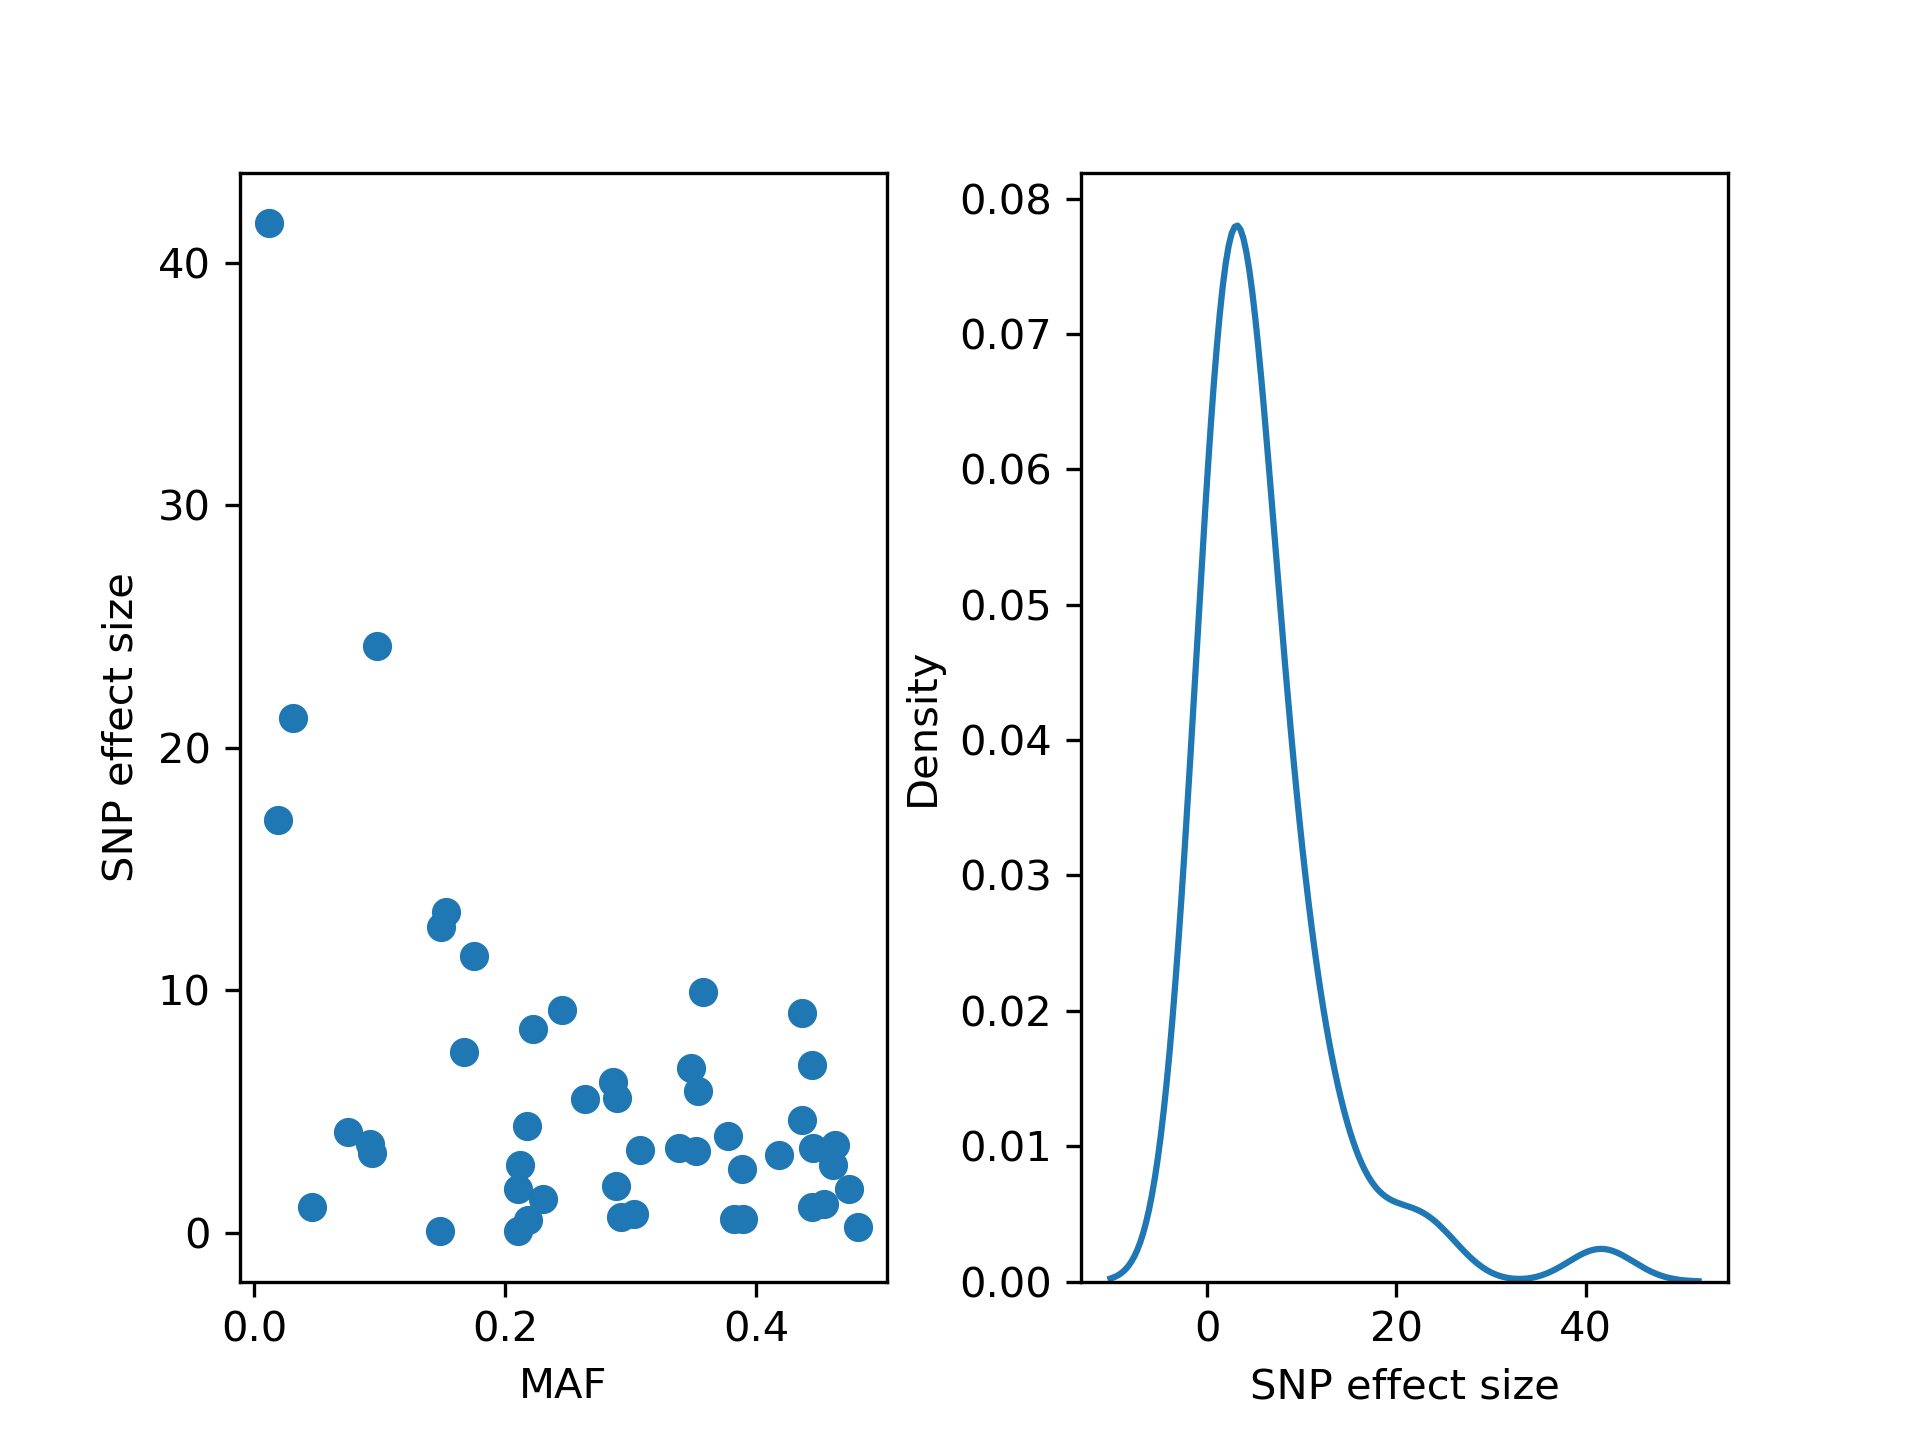
\includegraphics[width=0.95\textwidth]{figures/SNP_effects.png} \\ 
  \end{center}
  \caption{figures}
  \label{fig:all_figures}
\end{figure}

\begin{figure}
  \begin{center}
    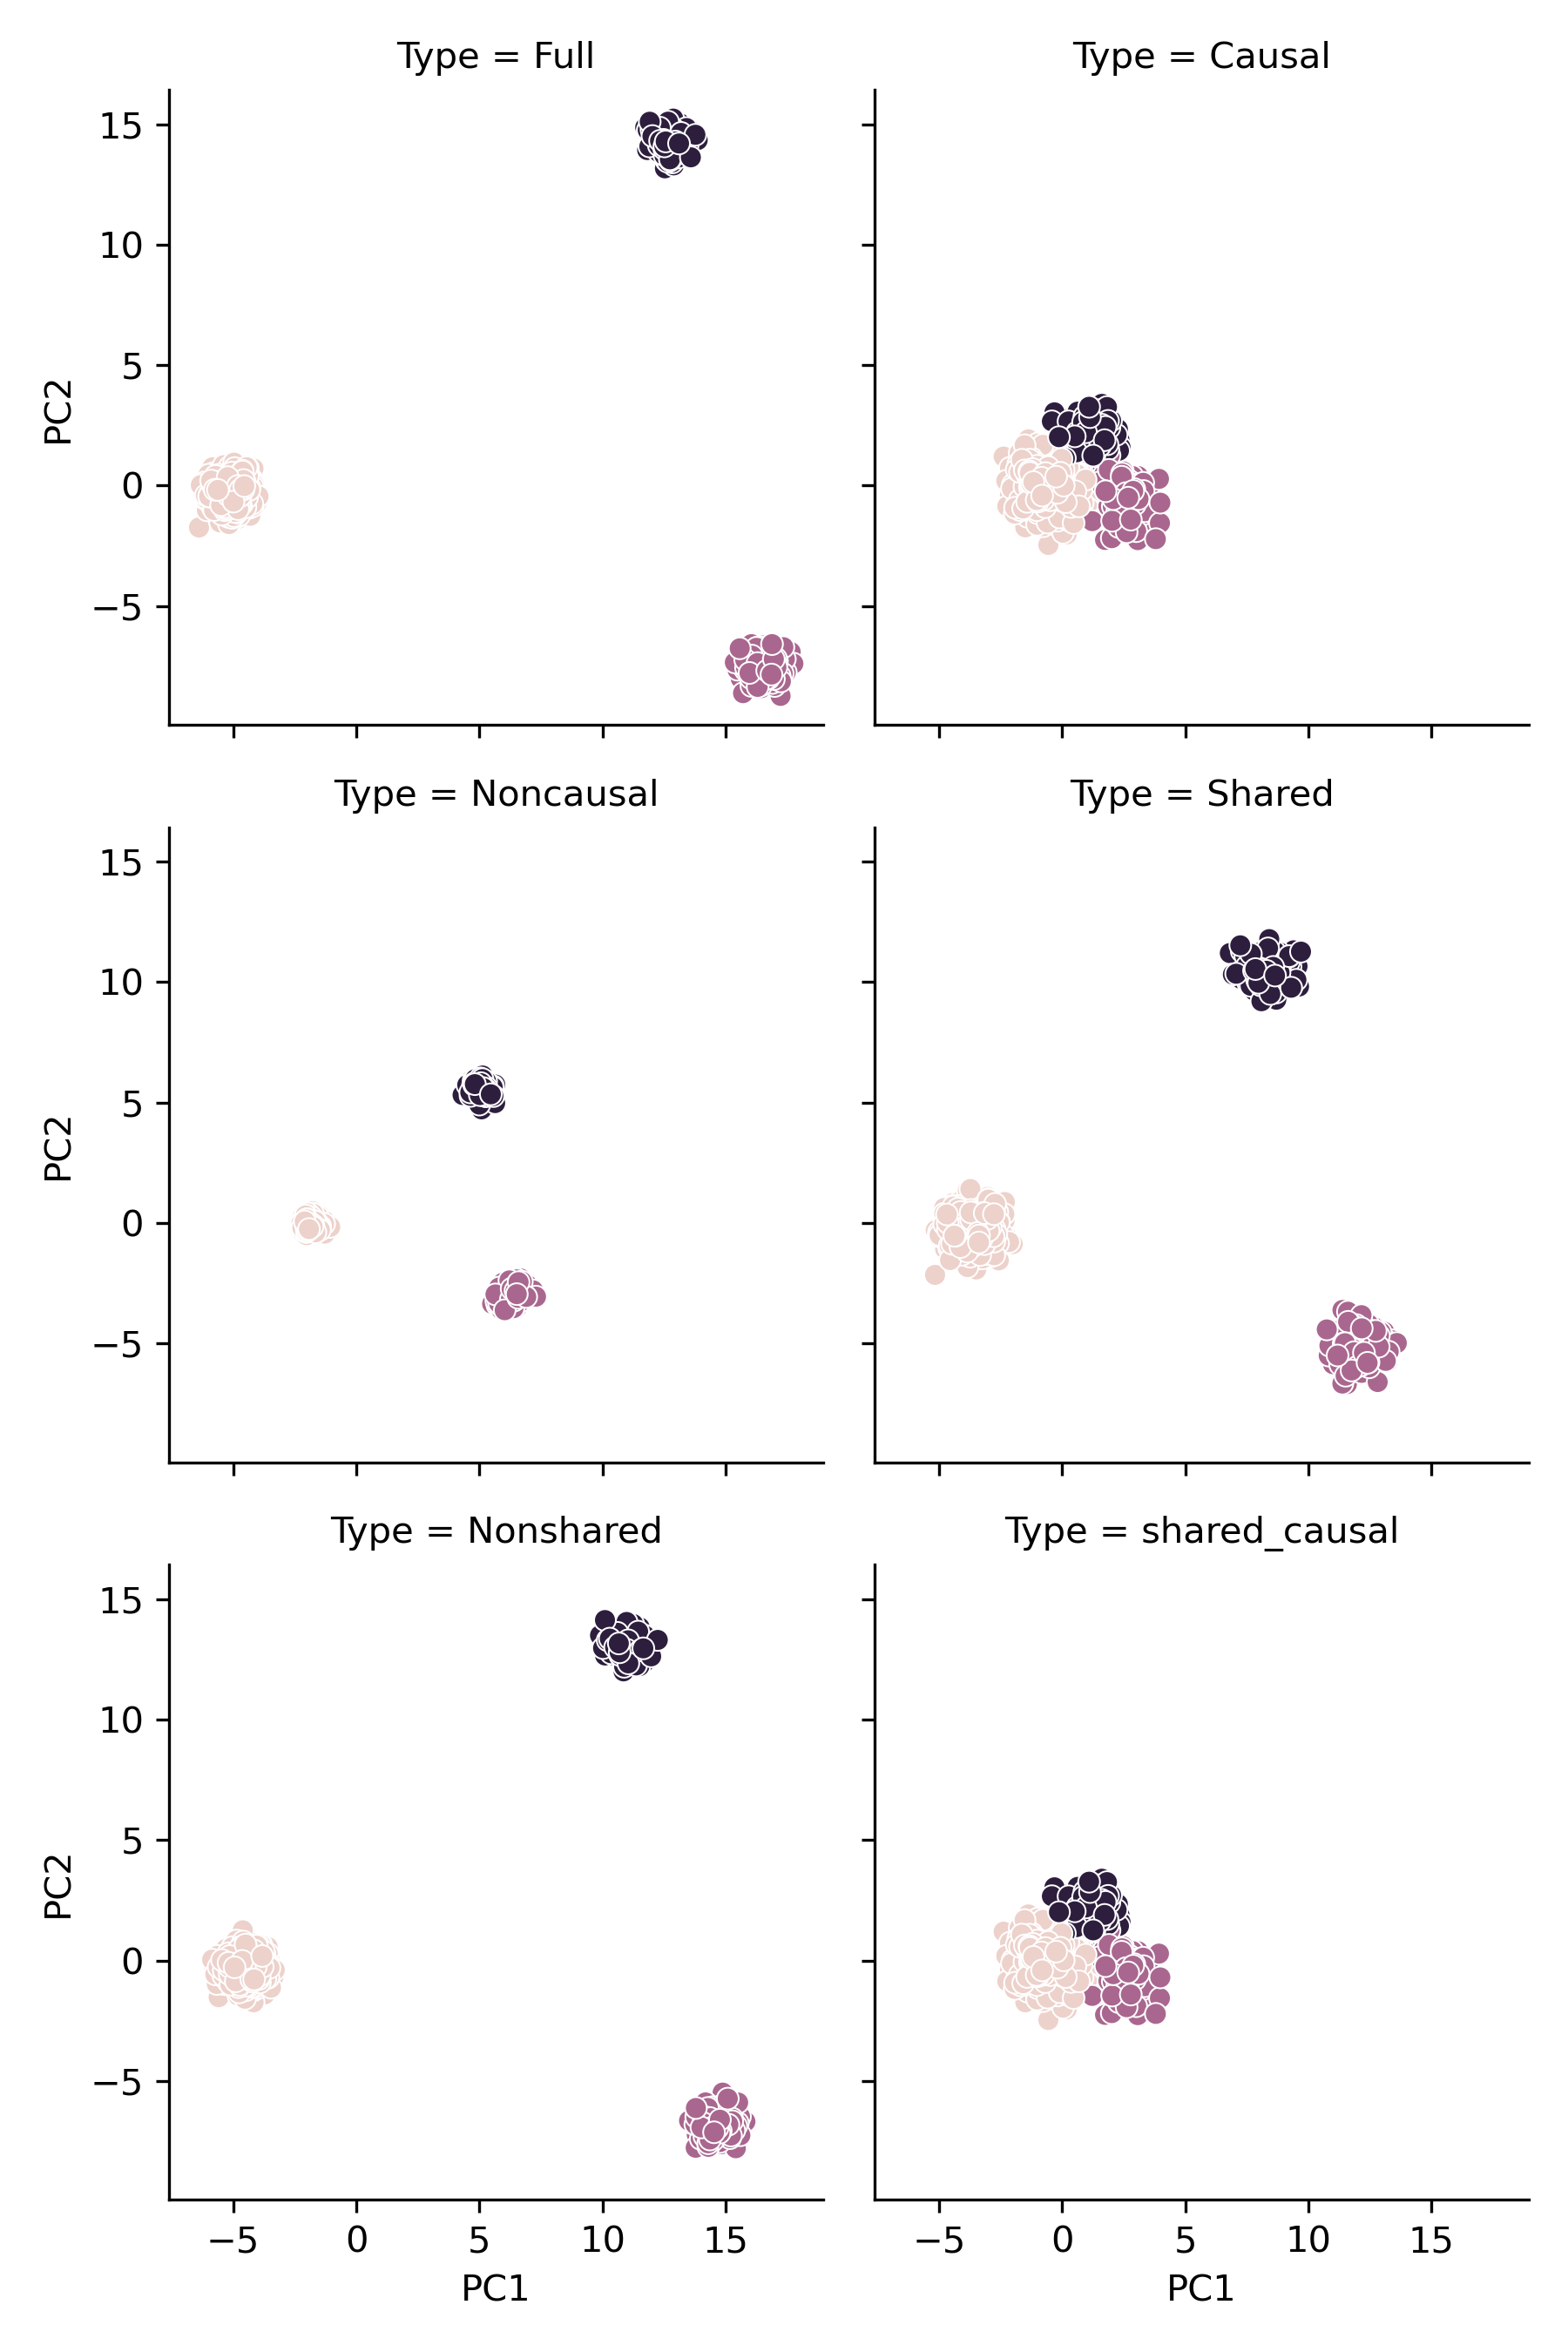
\includegraphics[width= 0.95\textwidth]{figures/genetic_clusters.png} \\
  \end{center}
  \caption{figures}
  \label{fig:all_figures}
\end{figure}
\begin{figure}
  \begin{center}
    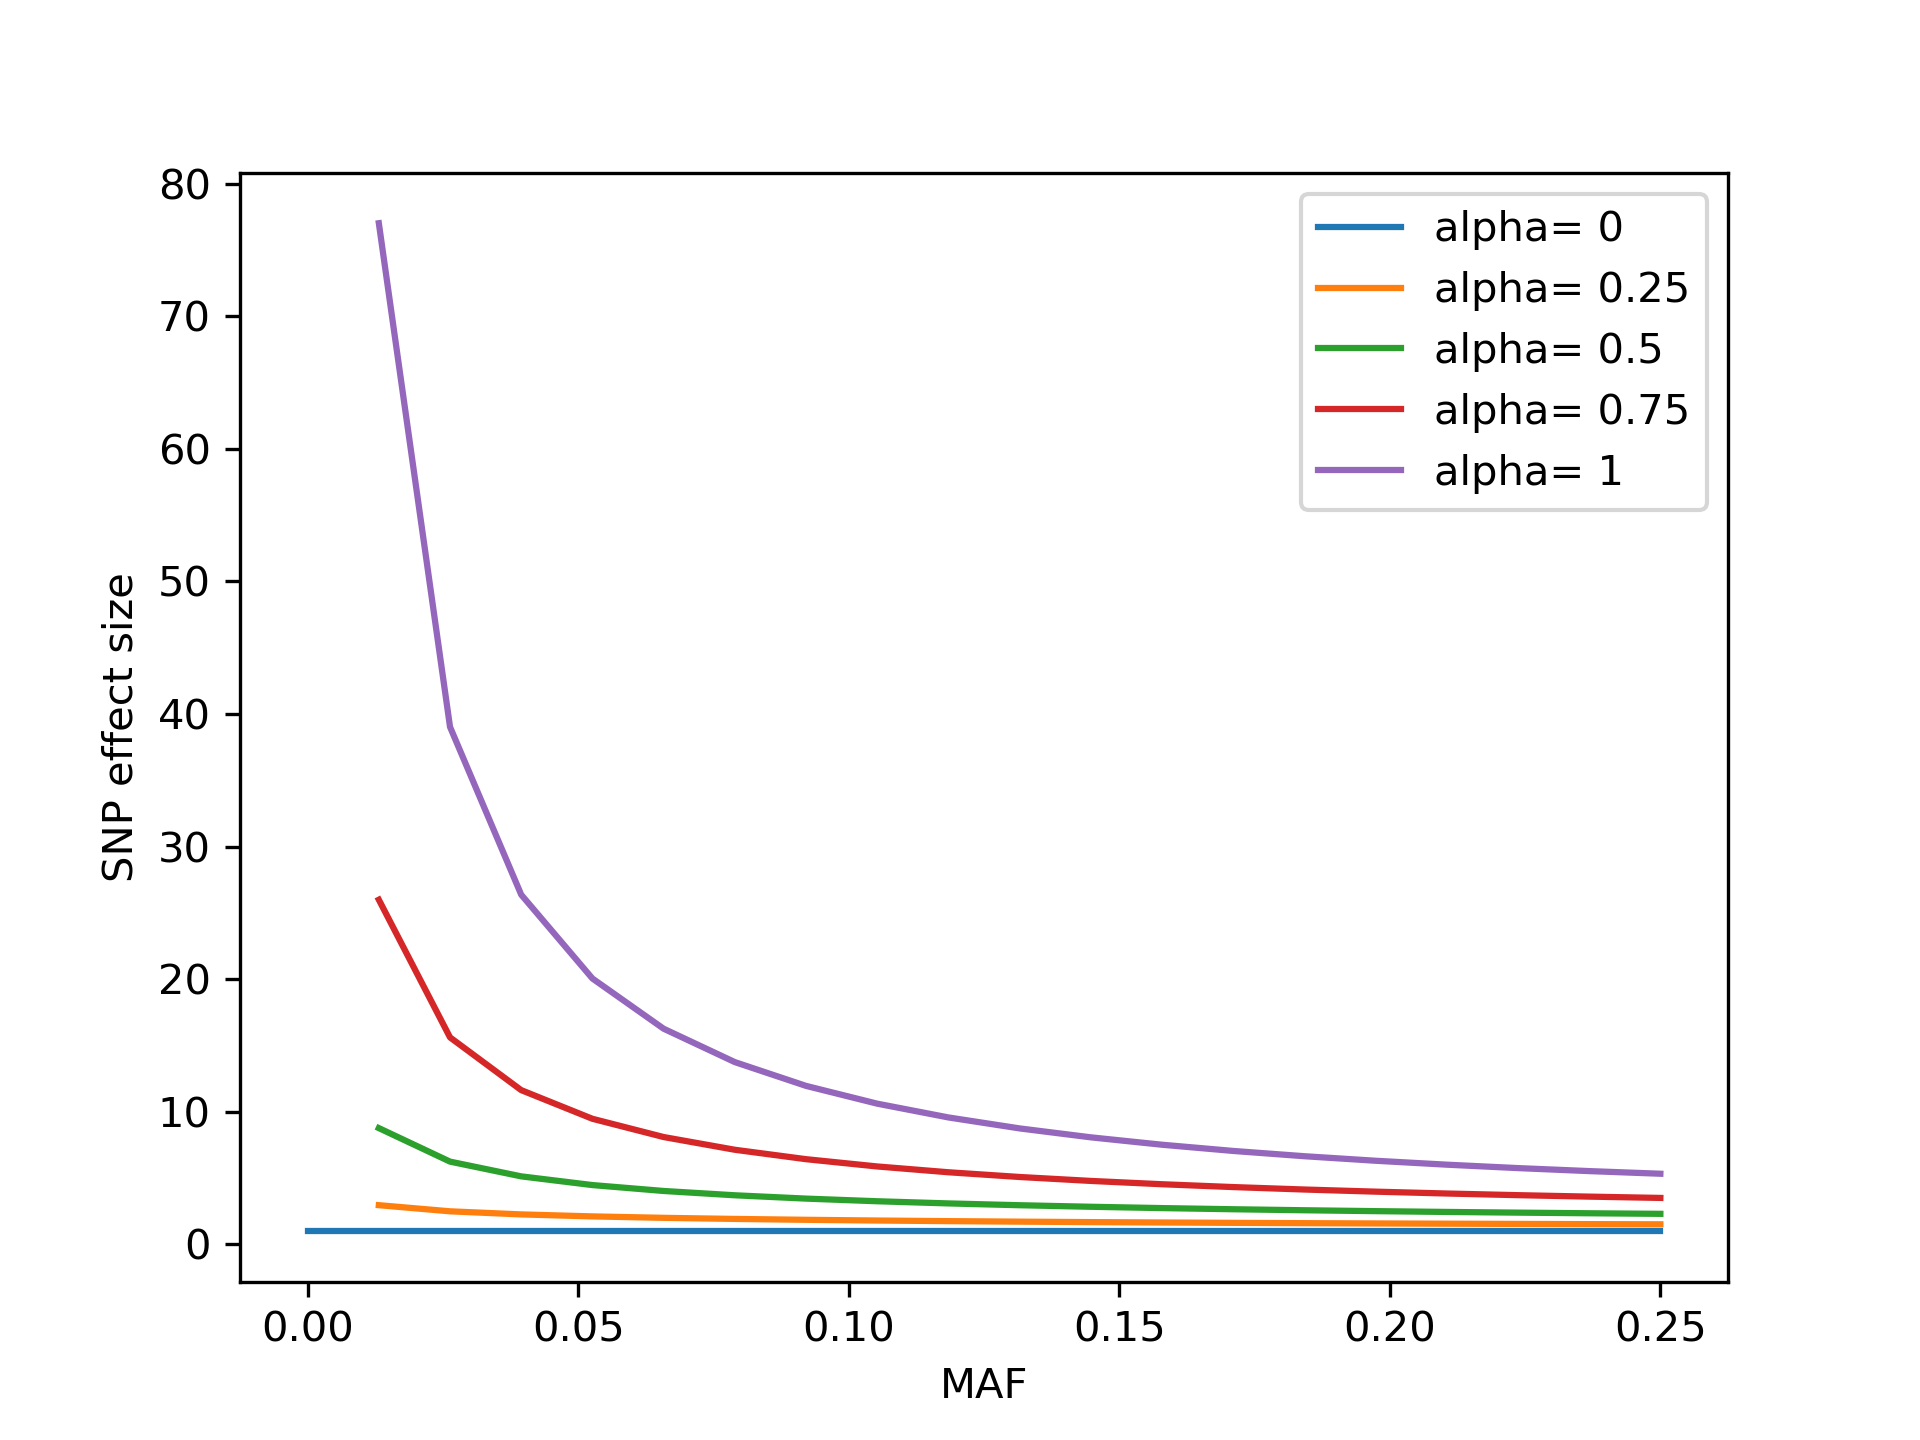
\includegraphics[width= 0.95\textwidth]{figures/SNPalphaControl.png}
  \end{center}
  \caption{figures}
  \label{fig:all_figures}
\end{figure}


\subsection{Simulating phenotypes}
% Genetic effects on phenotype: We discuss how the simulation class allows users to define the distribution of SNP effects and how they are assigned to genetic markers. We highlight the ability to incorporate observed frequencies of SNPs and their influence on the simulated phenotype.
% Incorporating other covariates: We explain how users can include additional covariates, such as environmental factors or demographic variables, to further refine the simulation of the phenotype.
% Introduction to utilizing existing genomic datasets: We highlight the flexibility of the simulation class to utilize preexisting genomic data, such as the "thousand genomes," as a starting point for simulating phenotypes.
% Loading and preprocessing genomic data: We describe the steps involved in loading and preprocessing the existing genomic dataset, including quality control procedures and data normalization.
% Genetic ancestry inference: We outline the methods used to infer genetic ancestries from the loaded dataset, allowing users to simulate phenotypes based on these inferred ancestries.
% Phenotype simulation based on genotypes: We explain how the loaded genotypes are utilized to simulate phenotypes, including the incorporation of SNP effects and the inclusion of other covariates if desired.
%Evaluating simulation accuracy: We discuss strategies for evaluating the accuracy and realism of the simulated phenotypes based on the existing genomic dataset, including comparison with observed phenotypes or external validation datasets.

The MASH toolbox provides a comprehensive framework for simulating phenotypes, allowing users to incorporate various factors such as SNP effects, unmodeled effects, continuous covariate effects, and confounding discrete variables.

To simulate the SNP effects, the MASH toolbox samples from a normal distribution. The variance of the distribution is specified by the desired heritability, allowing users to control the contribution of genetic factors to the phenotype. By sampling from a normal distribution, the toolbox captures the variability and range of SNP effects observed in real-world scenarios.

To incorporate additional unmodeled effects, the MASH toolbox simulates them as having a complementary variance to ensure the desired heritability. This approach ensures that the simulated phenotypes reflect the specified heritability and captures the presence of unaccounted factors that contribute to phenotypic variation.

For continuous covariate effects, the MASH toolbox simulates them as independent and identically distributed (IID) normal variables. This modeling approach allows users to introduce continuous covariates that may influence the phenotype while avoiding confounding with other factors.

In the case of confounding discrete variables, the MASH toolbox offers flexibility in simulating their effects. Users have the option to simulate the effects of each level of the variable either from a normal distribution or by specifying a fixed uniform set of values. Once the effects are simulated, the toolbox randomly assigns subjects to each level of the confounding variable, reflecting the presence of confounding factors in the simulated phenotypes.

\subsection{Additional tools for SNP-heritability estimation}
% Introduction to SNP-heritability estimation: We provide a brief overview of SNP-heritability estimation and its importance in understanding the genetic contribution to phenotypic variation.
% Site adjustment methods:

% COMBAT: We describe the COMBAT method, which is included in the toolbox, for adjusting site effects in multi-population genetics studies. We explain the underlying statistical framework and how it helps mitigate potential confounding due to site-specific differences.

% Meta-analysis estimation:

% Method overview: We introduce the meta-analysis estimation method available in the toolbox for combining SNP-heritability estimates across multiple populations or studies. We outline the steps involved in conducting meta-analysis and highlight its benefits in improving the accuracy and generalizability of SNP-heritability estimates.

% REML estimation using GCTA:

% Leveraging GCTA: We explain how the toolbox incorporates REML estimation using GCTA (Genome-wide Complex Trait Analysis) for estimating SNP-heritability. We describe the GCTA software and its application in estimating genetic variance components from genome-wide data.
% Methodology and implementation: We outline the underlying methodology of REML estimation and how it is implemented in the toolbox, including the necessary input data and parameters.

% Integration with simulation framework:

% Seamless integration: We highlight the seamless integration of these SNP-heritability estimation tools with the simulation framework provided by the toolbox. This integration allows users to evaluate the accuracy and performance of the estimation methods using simulated phenotypes with known SNP-heritability values.
% Assessment of method performance: We discuss how the toolbox facilitates the assessment of these estimation methods under various simulation scenarios, allowing researchers to compare and evaluate their performance in different population contexts.
The MASH toolbox provides a suite of additional tools for SNP-heritability estimation, allowing researchers to assess the contribution of genetic factors to phenotypic variation in multi-ancestry studies. These tools include site adjustment methods such as COMBAT, meta-analysis estimation, and REML estimation using GCTA.

Site adjustment methods are crucial in multi-site studies to account for potential site-specific effects that may introduce bias in SNP-heritability estimation. The MASH toolbox incorporates the popular COMBAT method, which effectively removes site effects and harmonizes the data across different study sites. By utilizing COMBAT, researchers can mitigate the confounding effects of site-specific variations and obtain more accurate estimates of SNP-heritability.

Meta-analysis estimation is another essential tool provided by the MASH toolbox. It enables researchers to combine results from multiple independent studies to increase statistical power and improve the estimation of SNP-heritability. The toolbox implements state-of-the-art meta-analysis methods, allowing for the integration of findings across diverse populations and study designs.

Furthermore, the MASH toolbox offers REML estimation using GCTA (Genome-wide Complex Trait Analysis). This powerful method utilizes genome-wide SNP data to estimate the proportion of phenotypic variance explained by genetic factors. By implementing GCTA, researchers can accurately estimate the SNP-heritability of the simulated phenotypes, providing valuable insights into the genetic architecture underlying complex traits.

The estimators included in the MASH toolbox have been extensively validated through comprehensive simulation studies. These studies have demonstrated the unbiasedness and robustness of the estimators, ensuring the reliability and accuracy of the SNP-heritability estimates obtained. By leveraging these tools, researchers can gain a deeper understanding of the genetic contributions to phenotypic variation in multi-ancestry populations and make informed conclusions about the heritability of specific traits.

\subsection{Accessibility and Integration}
The MASH toolbox has been designed with a strong emphasis on accessibility and ease of integration into researchers' workflows. It provides multiple ways for researchers to utilize the toolbox, including both Python and Bash interfaces.

By offering a Python interface, the MASH toolbox enables researchers to seamlessly integrate its functionalities into their existing Python-based analysis pipelines. Python is widely used in the scientific community for data analysis and has a rich ecosystem of libraries and tools. This integration allows researchers to leverage the MASH toolbox alongside other popular Python packages, facilitating a comprehensive analysis workflow.

Furthermore, the MASH toolbox also provides a Bash interface, allowing researchers to access its capabilities through command-line scripting. This flexibility in accessing the toolbox expands its usability to a broader audience, including researchers who prefer working with command-line tools or have established workflows that rely on Bash scripting.

\section{Results}\label{sec:results}
\begin{itemize}
  \item Comparison to GCTA
  \item A simulated example
  \item could do a bootstrapping example
  \item look for other simulation packages
\end{itemize}

\section{Discussion}\label{sec:discussion}

The MASH toolbox represents a significant advancement in the field of multi-ancestry, multi-site data simulation and analysis. By providing a comprehensive set of tools for simulating genetic ancestries, phenotypes, and estimating SNP-heritability, the toolbox addresses the need for standardized and semi-realistic simulations in multi-ancestry studies.

The toolbox's ability to simulate minimally complex, yet realistic multi-ancestry scenarios with confounding covariates, such as site effects, allows researchers to generate simulations that closely resemble real-world populations. Moreover, the flexibility to control heritability both at the individual ancestry level and collectively enhances the versatility of the toolbox for various research applications.

The validation of the estimators included in the toolbox through extensive simulation studies ensures their unbiasedness and reliability in estimating SNP-heritability. The toolbox also incorporates established methods for site adjustment, meta-analysis, and REML estimation using GCTA, providing researchers with robust tools to analyze and interpret multi-ancestry datasets.

The accessibility of the MASH toolbox through both Python and Bash interfaces enhances its usability and integration into researchers' workflows. The availability of a Python interface allows researchers to seamlessly incorporate the toolbox's functionalities into their existing Python-based analysis pipelines. Python is widely adopted in the scientific community and offers a comprehensive ecosystem of libraries and tools for data analysis. By integrating the MASH toolbox with popular Python packages, researchers can leverage its capabilities alongside other established tools, promoting a holistic and efficient analysis workflow.
Overall, the MASH toolbox empowers researchers to conduct sophisticated simulations and accurately assess the genetic contributions to phenotypic variation in multi-ancestry studies. By facilitating the generation of realistic simulations and offering advanced estimation methods, the toolbox opens up new avenues for understanding the complexities of genetic architecture in diverse populations and enables more reliable analyses of multi-ancestry datasets.

\backmatter

\bmhead{Supplementary information}

If your article has accompanying supplementary file/s please state so here. 

Authors reporting data from electrophoretic gels and blots should supply the full unprocessed scans for key as part of their Supplementary information. This may be requested by the editorial team/s if it is missing.

Please refer to Journal-level guidance for any specific requirements.

\bmhead{Acknowledgments}

Acknowledgments are not compulsory. Where included they should be brief. Grant or contribution numbers may be acknowledged.

Please refer to Journal-level guidance for any specific requirements.

\section*{Declarations}

Some journals require declarations to be submitted in a standardised format. Please check the Instructions for Authors of the journal to which you are submitting to see if you need to complete this section. If yes, your manuscript must contain the following sections under the heading `Declarations':

\begin{itemize}
\item Funding
\item Conflict of interest/Competing interests (check journal-specific guidelines for which heading to use)
\item Ethics approval 
\item Consent to participate
\item Consent for publication
\item Availability of data and materials
\item Code availability 
\item Authors' contributions
\end{itemize}

\noindent
If any of the sections are not relevant to your manuscript, please include the heading and write `Not applicable' for that section. 

%%===================================================%%
%% For presentation purpose, we have included        %%
%% \bigskip command. please ignore this.             %%
%%===================================================%%
\bigskip
\begin{flushleft}%
Editorial Policies for:

\bigskip\noindent
Springer journals and proceedings: \url{https://www.springer.com/gp/editorial-policies}

\bigskip\noindent
Nature Portfolio journals: \url{https://www.nature.com/nature-research/editorial-policies}

\bigskip\noindent
\textit{Scientific Reports}: \url{https://www.nature.com/srep/journal-policies/editorial-policies}

\bigskip\noindent
BMC journals: \url{https://www.biomedcentral.com/getpublished/editorial-policies}
\end{flushleft}

\begin{appendices}

\section{Section title of first appendix}\label{secA1}

An appendix contains supplementary information that is not an essential part of the text itself but which may be helpful in providing a more comprehensive understanding of the research problem or it is information that is too cumbersome to be included in the body of the paper.

%%=============================================%%
%% For submissions to Nature Portfolio Journals %%
%% please use the heading ``Extended Data''.   %%
%%=============================================%%

%%=============================================================%%
%% Sample for another appendix section			       %%
%%=============================================================%%

%% \section{Example of another appendix section}\label{secA2}%
%% Appendices may be used for helpful, supporting or essential material that would otherwise 
%% clutter, break up or be distracting to the text. Appendices can consist of sections, figures, 
%% tables and equations etc.

\end{appendices}

%%===========================================================================================%%
%% If you are submitting to one of the Nature Portfolio journals, using the eJP submission   %%
%% system, please include the references within the manuscript file itself. You may do this  %%
%% by copying the reference list from your .bbl file, paste it into the main manuscript .tex %%
%% file, and delete the associated \verb+\bibliography+ commands.                            %%
%%===========================================================================================%%

\bibliography{sn-bibliography}% common bib file
%% if required, the content of .bbl file can be included here once bbl is generated
%%\input sn-article.bbl


\end{document}
